\documentclass[10pt]{article}
\usepackage[letterpaper]{geometry}
\geometry{verbose,tmargin=1in,bmargin=1in,lmargin=1in,rmargin=1in}
\usepackage{setspace}
\usepackage{ragged2e}
\usepackage{color}
\usepackage{titlesec}
\usepackage{graphicx}
\usepackage{float}
\usepackage{mathtools}
\usepackage{amsmath}
\usepackage[font=small,labelfont=bf,labelsep=period]{caption}
\usepackage[english]{babel}
\usepackage{indentfirst}
\usepackage{array}
\usepackage{makecell}
\usepackage[usenames,dvipsnames]{xcolor}
\usepackage{multirow}
\usepackage{tabularx}
\usepackage{arydshln}
\usepackage{caption}
\usepackage{subcaption}
\usepackage{xfrac}
\usepackage{etoolbox}
\usepackage{cite}
\usepackage{url}
\usepackage{dcolumn}
\usepackage{hyperref}
\usepackage{courier}
\usepackage{url}
\usepackage{esvect}
\usepackage{commath}
\usepackage{verbatim} % for block comments
\usepackage{enumitem}
\usepackage{hyperref} % for clickable table of contents
\usepackage{braket}
\usepackage{titlesec}
\usepackage{booktabs}
\usepackage{gensymb}
\usepackage{longtable}
\usepackage{listings}
\lstset{
    frame=single,
    breaklines=true,
    postbreak=\raisebox{0ex}[0ex][0ex]{\ensuremath{\color{red}\hookrightarrow\space}}
}

% for circled numbers
\usepackage{tikz}
\newcommand*\circled[1]{\tikz[baseline=(char.base)]{
            \node[shape=circle,draw,inner sep=2pt] (char) {#1};}}


\titleclass{\subsubsubsection}{straight}[\subsection]

% define new command for triple sub sections
\newcounter{subsubsubsection}[subsubsection]
\renewcommand\thesubsubsubsection{\thesubsubsection.\arabic{subsubsubsection}}
\renewcommand\theparagraph{\thesubsubsubsection.\arabic{paragraph}} % optional; useful if paragraphs are to be numbered

\titleformat{\subsubsubsection}
  {\normalfont\normalsize\bfseries}{\thesubsubsubsection}{1em}{}
\titlespacing*{\subsubsubsection}
{0pt}{3.25ex plus 1ex minus .2ex}{1.5ex plus .2ex}

\makeatletter
\renewcommand\paragraph{\@startsection{paragraph}{5}{\z@}%
  {3.25ex \@plus1ex \@minus.2ex}%
  {-1em}%
  {\normalfont\normalsize\bfseries}}
\renewcommand\subparagraph{\@startsection{subparagraph}{6}{\parindent}%
  {3.25ex \@plus1ex \@minus .2ex}%
  {-1em}%
  {\normalfont\normalsize\bfseries}}
\def\toclevel@subsubsubsection{4}
\def\toclevel@paragraph{5}
\def\toclevel@paragraph{6}
\def\l@subsubsubsection{\@dottedtocline{4}{7em}{4em}}
\def\l@paragraph{\@dottedtocline{5}{10em}{5em}}
\def\l@subparagraph{\@dottedtocline{6}{14em}{6em}}
\makeatother

\newcommand{\volume}{\mathop{\ooalign{\hfil$V$\hfil\cr\kern0.08em--\hfil\cr}}\nolimits}

\setcounter{secnumdepth}{4}
\setcounter{tocdepth}{4}
\begin{document}

\title{ME 280a: HW 2}
\author{April Novak}

\maketitle

\section{Introduction and Objectives}

The purpose of this study is to solve a simple finite element (FE) problem and perform a convergence study to determine the number of elements needed to reach a particular error relative to an analytical solution for different shape function orders. The Galerkin FE method is used, which for certain classes of problems possesses the ``best approximation property,'' a characteristic that signifies that the FE solution obtained is the best possible solution for a given mesh refinement and choice of shape functions. The mathematical procedure and numerical implementation is described in Section \ref{sec:Procedure}.

\section{Procedure}
\label{sec:Procedure}

This section details the problem statement and mathematical method used for solving the problem.

\subsection{Problem Statement}

This section describes the mathematical process used to solve the following problem:

\begin{equation}
\label{eq:Problem}
\begin{aligned}
\frac{d}{dx}\left(E(x)\frac{du}{dx}\right)=xk^3\cos{\left(\frac{2\pi kx}{L}\right)}\\
\frac{d}{dx}\left(\frac{du}{dx}\right)=\frac{1}{E}xk^3\cos{(\gamma x)}\\
\end{aligned}
\end{equation}

where \(E\) is the modulus of elasticity, \(u\) is the solution, \(k\) is a known constant, \(L\) is the problem domain length, and \(x\) is the spatial variable. For simplicity, a constant \(\gamma=2\pi k/L\) is defined, and it has been assumed that \(E\) is a constant. In order to verify that the program functions correctly, the FE solution to Eq. \eqref{eq:Problem} will be compared with the analytical solution to Eq. \eqref{eq:Problem}. To determine the analytical solution, integrate Eq. \eqref{eq:Problem} once to obtain:

\begin{equation}
\label{eq:Problem2}
\frac{du}{dx}=\frac{k^3}{E}\left\lbrack \frac{x}{\gamma}\sin{(\gamma x)}+\frac{1}{\gamma^2}\cos{(\gamma x)}\right\rbrack+C_1
\end{equation}

It has been assumed that \(E\) is not a function of \(x\), and hence can be treated as constant in the integration. Integrating once more:

\begin{equation}
\label{eq:Problem3}
u(x)=\frac{1}{E}\left\lbrack\frac{-xk^3}{\gamma^2}\cos{(\gamma x)}+\frac{2k^3}{\gamma^3}\sin{(\gamma x)}\right\rbrack+C_1x+C_2
\end{equation}

The boundary conditions for this problem are Dirichlet at both endpoints, such that:

\begin{equation}
\begin{aligned}
u(0)=3\\
u(L)=-1\\
\end{aligned}
\end{equation}

By applying these boundary conditions:

\begin{equation}
\label{eq:BC}
\begin{aligned}
C_1=\frac{1}{L}\left\lbrack(-1)E+\frac{Lk^3}{\gamma^2}\cos{(\gamma L)}-\frac{2k^3}{\gamma^3}\sin{(\gamma L)}-C_2\right\rbrack\\
C_2=3\\
\end{aligned}
\end{equation}

The purpose of this assignment is to solve Eq. \eqref{eq:Problem} with the finite element method (FEM) and then to determine how many elements are needed to obtain a specified error as a function of the order of the shape functions. The solutions for various numbers of elements will also be compared to illustrate how increasing the number of elements ``hones in'' on the analytical solution. In addition, the convergence rates of the different shape element orders will be plotted to determine the relationship between element order and the rate at which the error decreases as a function of the mesh spacing.

\subsection{Finite Element Implementation}

The Galerkin FEM achieves the best approximation property by approximating the true solution \(u(x)\) as \(u^N(x)\), where both \(u^N(x)\) and the test function \(\psi\) are expanded in the same set of \(N\) basis functions \(\phi\):

\begin{equation}
\label{eq:approx}
\begin{aligned}
u\approx u^N=\sum_{j=1}^{N}a_j\phi_j\\
\psi=\sum_{i=1}^{N}b_i\phi_i\\
\end{aligned}
\end{equation}

Galerkin's method is stated as:

\begin{equation}
r^N\cdot u^N=0
\end{equation}

where \(r^N\) is the residual. Hence, to formulate the weak form to Eq. \eqref{eq:Problem}, multiply Eq. \eqref{eq:Problem} through by \(\psi\) and integrate over all space, \(d\Omega\).

\begin{equation}
\int_{\Omega}^{}\frac{d}{dx}\left(E(x)\frac{du}{dx}\right)\psi d\Omega-\int_{\Omega}^{}xk^3\cos{(\gamma x)}\psi d\Omega=0
\end{equation}

Applying integration by parts to the first term:

\begin{equation}
-\int_{\Omega}^{}E(x)\frac{du}{dx}\frac{d\psi}{dx}d\Omega+\int_{\partial\Omega}^{}E(x)\frac{du}{dx}\psi d(\partial\Omega)-\int_{\Omega}^{}xk^3\cos{(\gamma x)}\psi d\Omega=0
\end{equation}

where \(\partial\Omega\) refers to one dimension lower than \(\Omega\), which for this case refers to evaluation at the endpoints of the domain. Hence, for this particular 1-D problem, the above reduces to:

\begin{equation}
\begin{aligned}
-\int_{0}^{L}E(x)\frac{du}{dx}\frac{d\psi}{dx}dx+ E(x)\frac{du}{dx}\psi\biggr\vert_{0}^{L}-\int_{0}^{L}xk^3\cos{(\gamma x)}\psi dx=0\\
\int_{0}^{L}E(x)\frac{du}{dx}\frac{d\psi}{dx}dx=-\int_{0}^{L}xk^3\cos{(\gamma x)}\psi dx+E(x)\frac{du}{dx}\psi\biggr\vert_{0}^{L}\\
\end{aligned}
\end{equation}

Inserting the approximation described in Eq. \eqref{eq:approx}:

\begin{equation}
\begin{aligned}
\int_{0}^{L}E(x)\frac{d\left(\sum_{j=1}^{N}a_j\phi_j\right)}{dx}\frac{d\left(\sum_{i=1}^{N}b_i\phi_i\right)}{dx}dx=-\int_{0}^{L}xk^3\cos{(\gamma x)}\sum_{i=1}^{N}b_i\phi_idx+E(x)\frac{du}{dx}\sum_{i=1}^{N}b_i\phi_i\biggr\vert_{0}^{L}\\
\end{aligned}
\end{equation}

Recognizing that \(b_i\) appears in each term, the sum of the remaining terms must also equal zero (i.e. basically cancel \(b_i\) from each term).

\begin{equation}
\begin{aligned}
\int_{0}^{L}E(x)\frac{d\left(\sum_{j=1}^{N}a_j\phi_j\right)}{dx}\frac{d\phi_i}{dx}dx=-\int_{0}^{L}xk^3\cos{(\gamma x)}\phi_idx+E(x)\frac{du}{dx}\phi_i\biggr\vert_{0}^{L}\\
\end{aligned}
\end{equation}

This equation can be satisfied for each choice of \(j\), and hence can be reduced to:

\begin{equation}
\begin{aligned}
\int_{0}^{L}E(x)\frac{d\left(a_j\phi_j\right)}{dx}\frac{d\phi_i}{dx}dx=-\int_{0}^{L}xk^3\cos{(\gamma x)}\phi_idx+E(x)\frac{du}{dx}\phi_i\biggr\vert_{0}^{L}\\
\end{aligned}
\end{equation}

This produces a system of matrix equations of the form:

\begin{equation}
\label{eq:MatrixEqn}
\textbf{K}\vv{a}=\vv{F}
\end{equation}

where:

\begin{equation}
\begin{aligned}
\label{eq:SystemEquations}
K_{ij}=\int_{0}^{L}E(x)\frac{d\phi_i}{dx}\frac{d\phi_j}{dx}dx\\
a_j=a_j\\
F_i=-\int_{0}^{L}xk^3\cos{(\gamma x)}\phi_idx+E(x)\frac{du}{dx}\phi_i\biggr\vert_{0}^{L}\\
\end{aligned}
\end{equation}

where the second term in \(F_i\) is only applied at nodes that have Neumann boundary conditions (since \(\psi\) satisfies the homogeneous form of the essential boundary conditions). The above equation governs the entire domain. \(\textbf{K}\) is an \(n \times n\) matrix, where \(n\) is the number of global nodes. The solution is contained within \(\vv{a}\). This matrix system is solved in this assignment by simple Gaussian elimination, such that \(\vv{a}=\textbf{K}^{-1}\vv{F}\).

Quadrature is used to perform the numerical integration because it is much faster, and more general, than symbolic integration of the terms appearing in Eq. \eqref{eq:SystemEquations}. In order for these equations to be useful with Gaussian quadrature, they must be transformed to the master element which exists over \(-1\leq\xi\leq1\):

\begin{equation}
\label{eq:GoverningEqnsIsoparametric}
\begin{aligned}
K_{ij}=\int_{0}^{L}E(x)\frac{d\phi_i}{dx}\frac{d\phi_j}{dx}dx\rightarrow\int_{-1}^{1}E(x(\xi))\frac{d\phi_i}{dx}\frac{d\phi_j}{dx}dx\left(\frac{dx}{d\xi}\frac{dx}{d\xi}\frac{d\xi}{dx}\right)\rightarrow\int_{-1}^{1}E(x(\xi))\frac{d\phi_i}{d\xi}\frac{d\phi_j}{d\xi}dx\left(\frac{d\xi}{dx}\right)\\
a_j=a_j\\
F_i=-\int_{0}^{L}xk^3\cos{(\gamma x)}\phi_idx\rightarrow-\int_{-1}^{1}x(\xi)k^3\cos{(\gamma x(\xi))}\phi_i\frac{dx}{d\xi}d\xi\\
\end{aligned}
\end{equation} 

where the second term in \(F_i\) has been dropped because there are no Neumann boundary conditions in this assignment. Three different shape function orders are used in this assignment - linear, quadratic, and cubic. All of these shape functions are Lagrangian shape functions that are determined by requiring them to go to zero at all nodes except the node to which they pertain. For linear elements, the shape functions have the following form and derivative over the master element:

\begin{equation}
\begin{aligned}
\phi_1(\xi)=\frac{1-\xi}{2},\quad\frac{d\phi_1(\xi)}{d\xi}=-1/2\\
\phi_2(\xi)=\frac{1+\xi}{2}, \quad\frac{d\phi_2(\xi)}{d\xi}=+1/2\\
\end{aligned}
\end{equation}

For quadratic elements, the shape functions have the following form and derivative over the master element:

\begin{equation}
\begin{aligned}
\phi_1(\xi)=\frac{(\xi-1)\xi}{2},\quad\frac{d\phi_1(\xi)}{d\xi}=\xi-1/2\\
\phi_2(\xi)=(1-\xi)(1+\xi), \hspace{0.9cm}\frac{d\phi_2(\xi)}{d\xi}=-2\xi\\
\phi_3(\xi)=\frac{(\xi+1)\xi}{2}, \quad\frac{d\phi_3(\xi)}{d\xi}=\xi+1/2\\
\end{aligned}
\end{equation}

For cubic elements, the shape functions have the following form and derivative over the master element:

\begin{equation}
\begin{aligned}
\phi_1(\xi)=\frac{9}{16}\left\lbrack(1-\xi)(1/3-\xi)(-1/3-\xi)\right\rbrack, \quad \frac{d\phi_1(\xi)}{d\xi}=\frac{9}{16}\left(-3\xi^2+2\xi+\frac{1}{9}\right)\\
\phi_2(\xi)=\frac{-27}{16}\left\lbrack(1-\xi)(1/3-\xi)(-1-\xi)\right\rbrack, \quad \frac{d\phi_2(\xi)}{d\xi}=\frac{-27}{16}\left(-3\xi^2+\frac{2\xi}{3}+1\right)\\
\phi_3(\xi)=\frac{27}{26}\left\lbrack(1-\xi)(-1/3-\xi)(-1-\xi)\right\rbrack, \quad \frac{d\phi_3(\xi)}{d\xi}=\frac{27}{16}\left(-3\xi^2-\frac{2\xi}{3}+1\right)\\
\phi_4(\xi)=\frac{-9}{16}\left\lbrack(1/3-\xi)(-1/3-\xi)(-1-\xi)\right\rbrack, \quad \frac{d\phi_4(\xi)}{d\xi}=\frac{-9}{16}\left(-3\xi^2-2\xi+\frac{1}{9}\right)\\
\end{aligned}
\end{equation}

where the nodes are spaced equally over \(-1\leq\xi\leq1\) (i.e. nodes at \(\pm 1/3\)). The transformation from the physical domain (\(x\)) to the parent domain (\(\xi\)) is done with an isoparametric mapping:

\begin{equation}
\label{eq:Mapping}
x(\xi)=\sum_{i=1}^{N} X_i\phi_i(\xi)
\end{equation}

where \(X_i\) are the coordinates in each element. This mapping is performed for each element individually. The Jacobian \(dx/d\xi\) is obtain from Eq. \eqref{eq:Mapping} by differentiation:

\begin{equation}
\frac{dx(\xi)}{d\xi}=\sum_{i=1}^{N} X_i\frac{d\phi_i(\xi)}{d\xi}
\end{equation}

With all these transformations from the physical domain to the isoparametric domain, Gaussian quadrature can be used. The quadrature used depends on the order of the shape functions. An \(n\) point quadrature rule can exactly integrate a polynomial of order \(2n-1\). From Eq. \eqref{eq:GoverningEqnsIsoparametric}, the integrand in \(K_{ij}\) will be of order \((n-1)(n-1)\), while the integrand in \(F_i\) will be of (technically) infinite order since cosine is not a polynomial, and it would require a summation of an infinite number of polynomials to approximate cosine as a polynomial (i.e. Taylor series). Neglecting the presence of the cosine function, then the integrand in \(F_i\) would be of order \(n^2\). So, the selection of the order of the quadrature rule is not straightforward. Table \ref{table:orders} shows the order of the different matrices and vectors in the governing equations in order to guide the selection of a quadrature rule. The number of quadrature points is selected according to the desire to integrate correctly \(F_{i}\) (neglecting the cosine term), since this is more restrictive than correctly integrating the integrand in \(K_{ij}\). When applicable, the number of quadrature points is rounded up. 

\begin{table}[H]
\caption{Number of quadrature points needed for exact integration of terms appearing in Eq. \eqref{eq:GoverningEqnsIsoparametric}. The ``order of integrand in \(F_i\)'' neglects the order of the cosine term.}
\centering
\begin{tabular}{c c c c}
\hline\hline
\(\phi\) order & order of integrand in \(K_{ij}\) & order of integrand in \(F_{i}\) & Quadrature points needed\\ [0.5ex]
\hline
1 & 0 & 2 & 2\\
2 & 1 & 4 & 3\\
3 & 4 & 9 & 5\\
\hline
\end{tabular}
\label{table:orders}
\end{table}

Hence, for cubic shape functions, a five-point rule is used, for quadratic a three-point rule, and for linear a two-point rule. These Gauss-Legendre rules are as follows. For the two-point quadrature rule, the weights \(w\) and sampling points \(x\) are:

\begin{equation}
\begin{aligned}
w=[1.0, 1.0]\\
x=[-\sqrt{1/3}, \sqrt{1/3}]\\
\end{aligned}
\end{equation} 

For the three-point quadrature rule, the weights \(w\) and sampling points \(x\) are:

\begin{equation}
\begin{aligned}
w=[5/9, 8/9, 5/9]\\
x=[-\sqrt{3/5}, 0, \sqrt{3/5}]\\
\end{aligned}
\end{equation} 

For the five-point quadrature rule, the weights \(w\) and sampling points \(x\) are:

\begin{equation}
\begin{aligned}
w=\left\lbrack\frac{322-13\sqrt{70}}{900}, \frac{322+13\sqrt{70}}{900}, \frac{128}{225}, \frac{322+13\sqrt{70}}{900}, \frac{322-13\sqrt{70}}{900}\right\rbrack\\
x=\left\lbrack-\frac{1}{3}\sqrt{5+2\sqrt{10/7}}, -\frac{1}{3}\sqrt{5-2\sqrt{10/7}}, 0, \frac{1}{3}\sqrt{5-2\sqrt{10/7}}, \frac{1}{3}\sqrt{5+2\sqrt{10/7}}\right\rbrack\\
\end{aligned}
\end{equation} 

Transformation to the isoparametric domain therefore easily allows construction of the local stiffness matrix and local force matrix. The actual numerical algorithm computes the elemental \(k(i,j)\) and \(b(i)\) by looping over \(i, j\), and the quadrature points. Because each calculation is computed over a single element, a connectivity matrix is used to populate the global stiffness matrix and the global forcing vector with the elemental matrices and vectors. See the Appendix for the full code used in this assignment. After the global matrix and vector are formed, the global matrix has a banded-diagonal structure. 

In order to apply the boundary conditions within the numerical context of the finite element method, the matrix equation in Eq. \eqref{eq:MatrixEqn} must be rewritten to reflect that some of the nodal values are actually already specified through the Dirichlet boundary conditions. 

\begin{equation}
\label{eq:condensation}
\begin{bmatrix}
	K_{kk} & K_{ku}\\
	K_{uk} & K_{uu}\\
\end{bmatrix}
\begin{bmatrix}
	x_k\\
	x_u\\
\end{bmatrix}
=
\begin{bmatrix}
	F_k\\
	F_u\\
\end{bmatrix}
\end{equation}

where \(k\) indicates a known quantity (specified through a boundary condition) and \(u\) indicates an unknown quantity.   Explicitly expanding this equation gives:

\begin{equation}
\begin{aligned}
K_{kk}x_k+K_{ku}x_u=F_k\\
K_{uk}x_k+K_{uu}x_u=F_u\\
\end{aligned}
\end{equation}

Solving this matrix system is sometimes referred to as ``static condensation,'' since the original matrix system in Eq. \eqref{eq:MatrixEqn} must be separated into its components. The nodes at which Dirichlet conditions are specified are ``known,'' while all other nodes, including Neumann condition nodes, are ``unknown,'' since it is the value of \(u\) that we are looking to find at each node. The second of these equations is the one that is solved in this assignment, since there are no natural boundary conditions.

Once the solution is obtained by simple Gaussian elimination, the solution is transformed back to the physical domain (from the isoparametric domain) by solving a linear matrix system to determine the coefficients on the basis functions over each element (in the physical domain). For example, for a quadratic shape function, over one element with coordinates \(x_1, x_2,\) and \(x_3\), with solution values \(a_1, a_2,\) and \(a_3\), the following linear system solves for the coordinates on the shape function in the physical domain, in that element:

\begin{equation}
\label{eq:LinearSolve}
\begin{bmatrix}
1 & x_1 & x_1^2\\
1 & x_2 & x_2^2\\
1 & x_3 & x_3^2\\
\end{bmatrix}
\begin{bmatrix} A\\ B\\ C
\end{bmatrix}
=
\begin{bmatrix} a_1 \\ a_2 \\ a_3
\end{bmatrix}
\end{equation}

Each element is looped over to obtain the coefficients on the shape functions in the physical domain. This then transforms the solution back to the physical domain, and completes the FE solution.

\subsection{Error Estimates and Convergence Criteria}

The accuracy of the FE solution is estimated using the energy norm \(e^N\), defined as:

\begin{equation}
e^N=\frac{\|u-u^N\|}{\|u\|}
\end{equation}

where:

\begin{equation}
\|u\|=\sqrt{\int_{\Omega}^{}\frac{du}{dx}E\frac{du}{dx}}
\end{equation}

\begin{equation}
\|u-u^N\|=\sqrt{\int_{\Omega}^{}\frac{d(u-u^N)}{dx}E\frac{d(u-u^N)}{dx}}=\sqrt{\int_{\Omega}^{}\left(\frac{du}{dx}-\frac{du^N}{dx}\right)E\left(\frac{du}{dx}-\frac{du^N}{dx}\right)}
\end{equation}

The derivatives of the FE solution are determined according to:

\begin{equation}
\frac{du^N}{dx}=\frac{d}{dx}\sum_{j=1}^{N}a_j\phi_j(x)=\sum_{j=1}^{N}a_j\frac{d\phi_j(x)}{dx}=\sum_{j=1}^{N}a_j\frac{d\phi_j(x)}{d\xi}\frac{d\xi}{dx}
\end{equation}

while the derivative of the analytical solution is obtained from Eq. \eqref{eq:Problem2}. Convergence is defined to have been achieved for a given \(k\) and number of elements \(N\) once:

\begin{equation}
\label{eq:Convergence}
e^N=\frac{\|u-u^N\|}{\|u\|} \leq 0.04
\end{equation}

\subsection{Solution Results and Discussion}

Table \ref{table:orders} shows the number of elements needed to reach the tolerance given by Eq. \eqref{eq:Convergence} as a function of the polynomial order of the approximation functions. The higher the element order, the less elements that are needed to reach the specified convergence criteria, as expected. The higher the polynomial order of the shape functions, the more degrees of freedom that are available to capture the behavior of the true solution. 

It is important to take the results shown in Table \ref{table:orders} with a ``grain of salt'' because they depend on how exactly I compute the energy norm - I use \texttt{trapz()}, which is sensitive to the mesh I use. I use a very fine mesh, which is perhaps why the numbers of intervals over which I compute the integrals in the energy norm provides a lower energy norm than for students who use quadrature or the \(a^T\textbf{K}a\) method for computing the energy norm. 

\begin{table}[H]
\caption{Number of elements needed to reach a tolerance given by Eq. \eqref{eq:Convergence} based on the polynomial order of the approximating functions.}
\centering
\begin{tabular}{c c}
\hline\hline
\(\phi\) order & Number of elements needed\\ [0.5ex]
\hline
1 & 543\\
2 & 73\\
3 & 24\\
\hline
\end{tabular}
\label{table:orders}
\end{table}

\begin{figure}[H]
\centering
\begin{subfigure}{.48\textwidth}
  \centering
  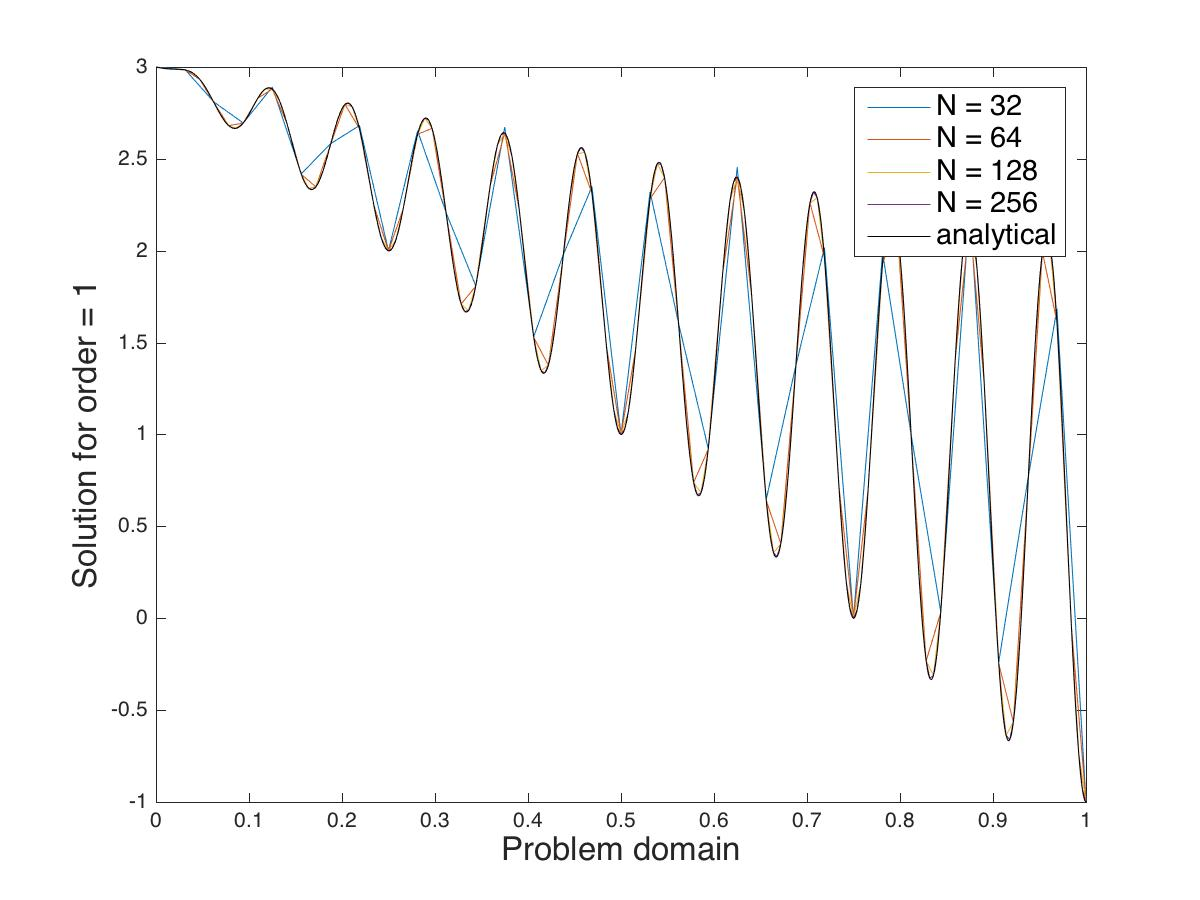
\includegraphics[width=1.0\linewidth]{Nplot_for_order_1.jpg}
  \caption{}
\end{subfigure}
\begin{subfigure}{.48\textwidth}
  \centering
  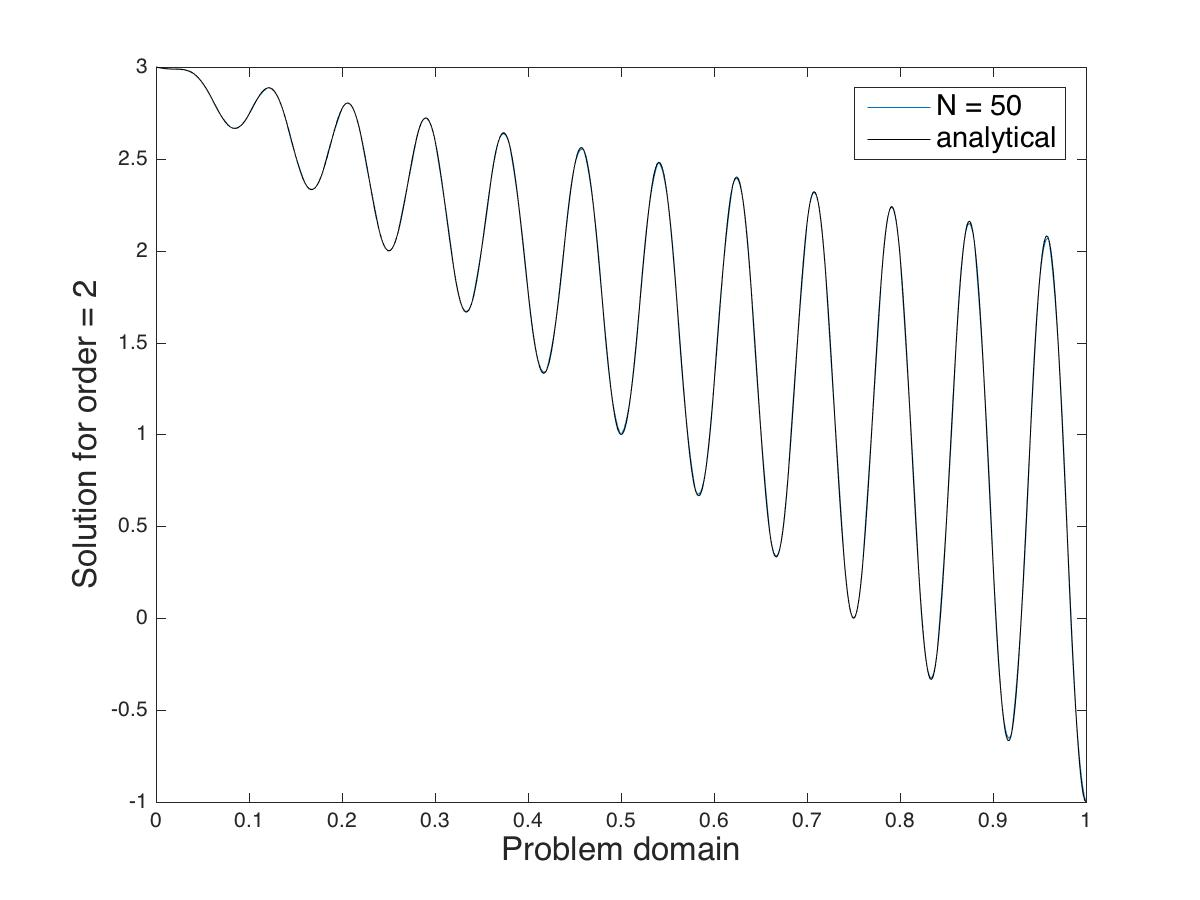
\includegraphics[width=1.0\linewidth]{Nplot_for_order_2.jpg}
  \caption{}
\end{subfigure}
\begin{subfigure}{.48\textwidth}
  \centering
  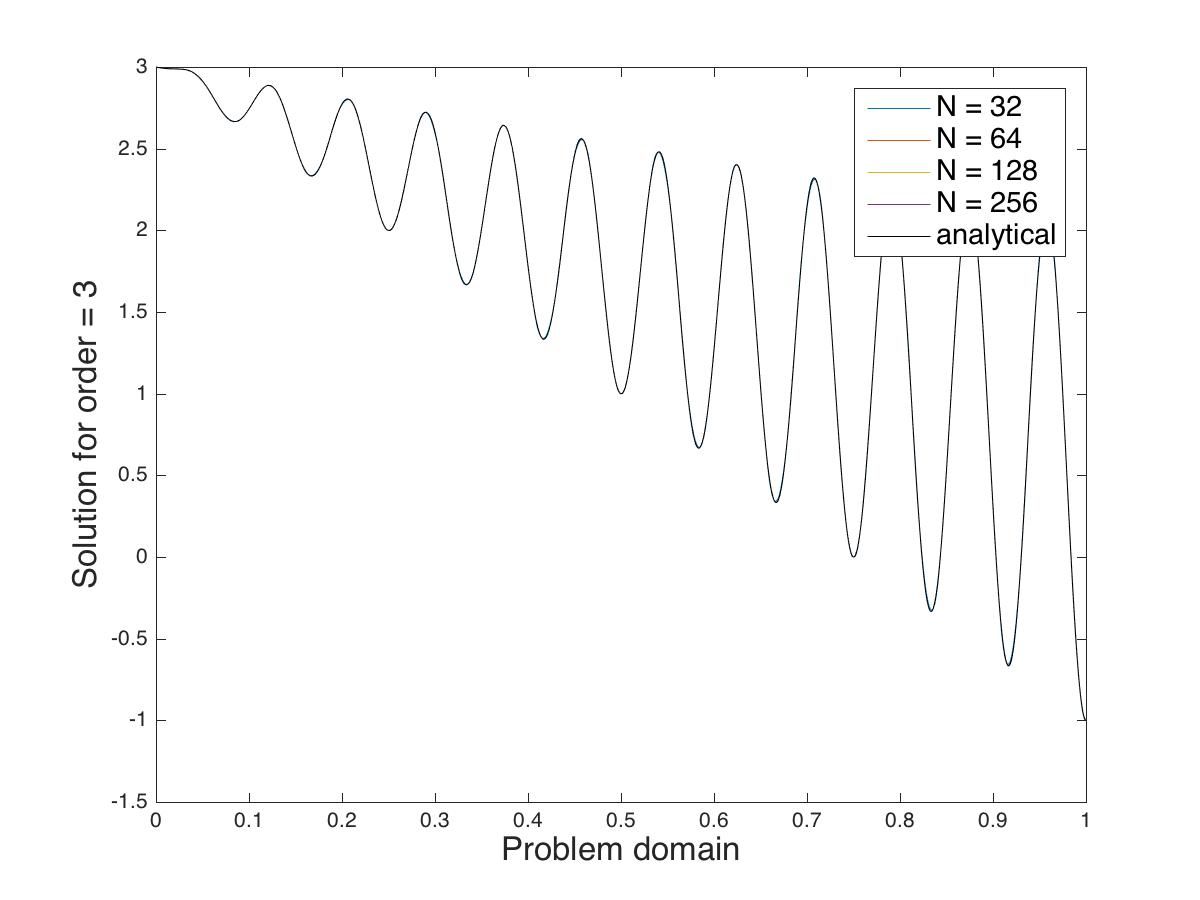
\includegraphics[width=1.0\linewidth]{Nplot_for_order_3.jpg}
  \caption{}
\end{subfigure}
\caption{Finite element and exact (analytical) solutions for \(N=16, 32, 64, 128, 256\) for (a) linear, (b) quadratic, and (c) cubic approximation functions.}
\label{fig:Nplots}
\end{figure}

Fig. \ref{fig:eN_vs_h} shows the error as a function of the element size \(h \equiv L/(\textrm{number of elements})\) for linear (order = 1), quadratic (order = 2), and cubic (order = 3) shape functions. As can be seen, the higher the approximation function order, the faster the energy norm reaches its asymptotic value. 

\begin{figure}[H]
  \centering
  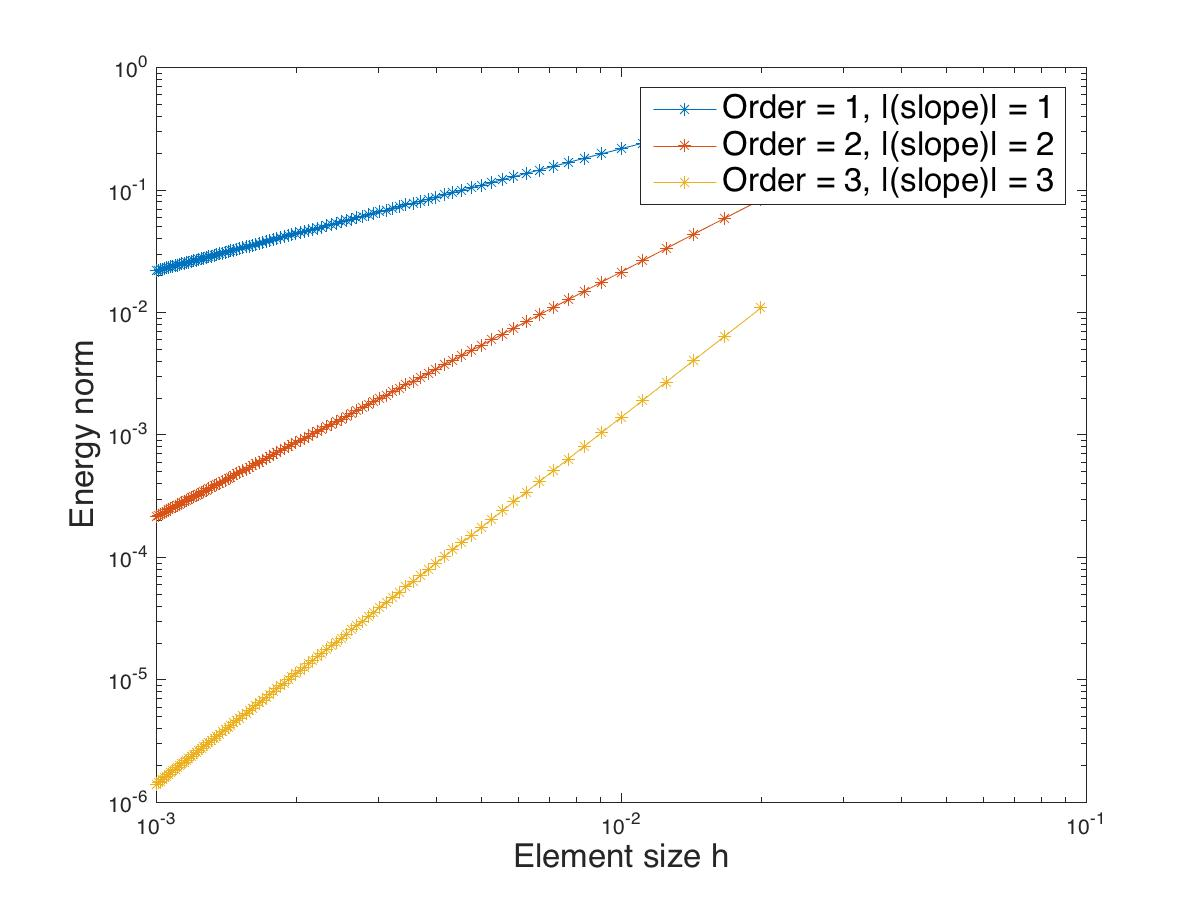
\includegraphics[width=13cm]{eN_vs_h.jpg}
  \caption{Energy norm \(e^N\) as a function of \(h\) for different polynomial orders.}
  \label{fig:eN_vs_h}
\end{figure}

Fig. \ref{fig:eN_vs_dof} essentially shows the same information as Fig. \ref{fig:eN_vs_h}, except that the independent variable is the number of degrees of freedom. For a linear element, there are two degrees of freedom, for a quadratic element there are three, and for a cubic element there are four. As can seen, the smaller the \(h\), or the greater the number of degrees of freedom, the lower the error when represented as the energy norm.

\begin{figure}[H]
  \centering
  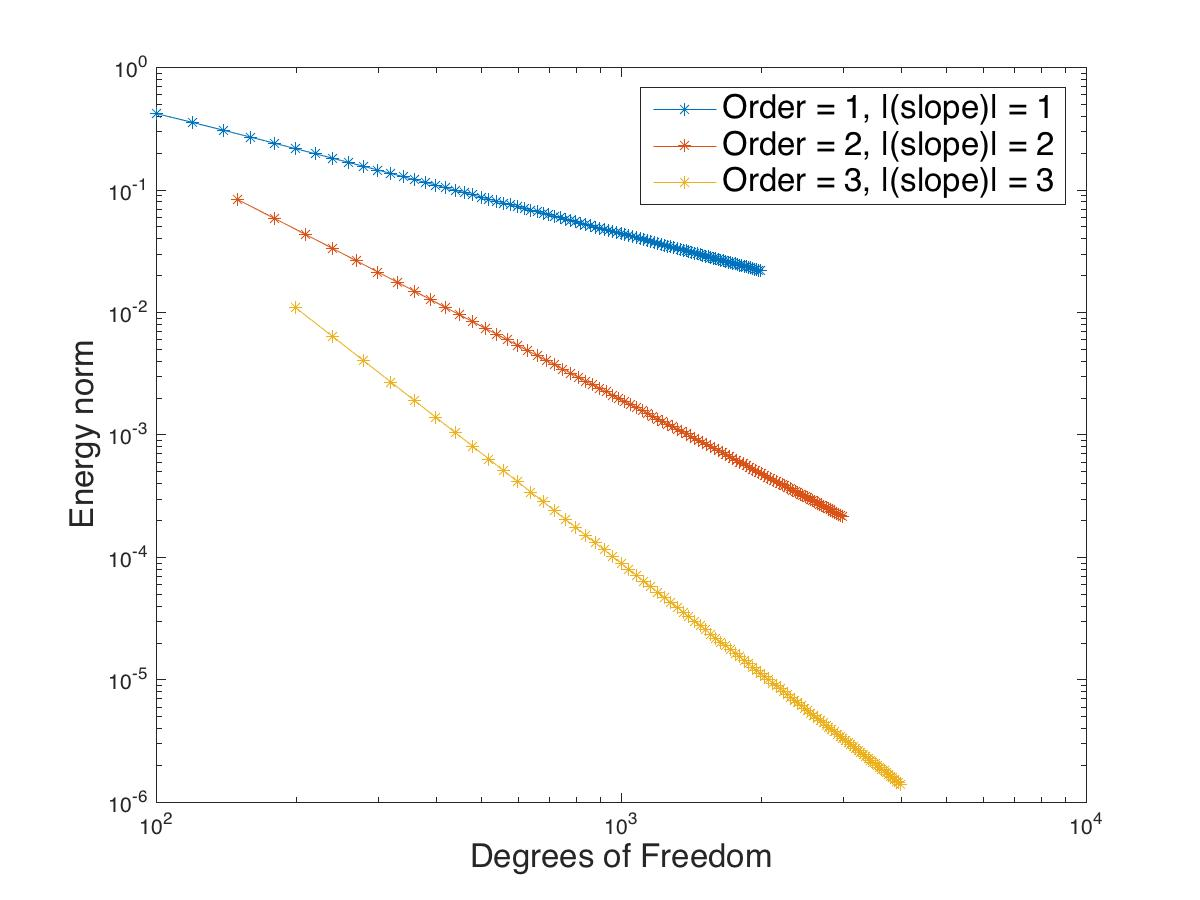
\includegraphics[width=13cm]{eN_vs_dof.jpg}
  \caption{Energy norm \(e^N\) as a function of the number of degrees of freedom for different polynomial orders.}
  \label{fig:eN_vs_dof}
\end{figure}

\section{Appendix}

This section contains the code used for this modeling. The main program is \texttt{FEProgram.m}, and functions perform specialized tasks for a high degree of modularity.

\subsection{\texttt{FEProgram.m}}
\lstinputlisting[language=Matlab]{FEProgram.m}

\subsection{\texttt{permutation.m}}
This function determines the permutation matrix for use with the connectivity matrix.
\lstinputlisting[language=Matlab]{permutation.m}

\subsection{\texttt{mesh.m}}
This function performs the meshing.
\lstinputlisting[language=Matlab]{mesh.m}

\subsection{\texttt{BCnodes.m}}
This function applies boundary conditions.
\lstinputlisting[language=Matlab]{BCnodes.m}

\subsection{\texttt{shapefunctions.m}}
This function contains the library of shape functions.
\lstinputlisting[language=Matlab]{shapefunctions.m}

\subsection{\texttt{quadrature.m}}
This function selects the quadrature rule.
\lstinputlisting[language=Matlab]{quadrature.m}

\subsection{\texttt{condensation.m}}
This function separates out the matrix equation as in Eq. \eqref{eq:condensation}.
\lstinputlisting[language=Matlab]{condensation.m}

\subsection{\texttt{postprocess.m}}
This function postprocesses the FE solution and transforms it back to the physical domain using a linear system solve as described in Eq. \eqref{eq:LinearSolve}.
\lstinputlisting[language=Matlab]{postprocess.m}


\end{document}